\section{Introduction}

A \emph{pangenome} models the full set of genomic elements in a given species or clade \cite{sigaux2000cancer}.
Pangenomics thus stands in contrast to standard genomics by emphasizing the sum total of available genomic information over a particular consensus model of the genome.
By considering the pangenome during bioinformatic analyses, researchers can hope to remove bias towards any specific genome or haploid genome model that might occur during diverse stages of data processing.
%, analyse also minor alleles inevitably missing from such linear models, and incorporate information about genomic variation directly into their study.
%Pangenomic reference systems thus e single canonical version of the genome of a given species, but a widely-represenative collection of sequences.

This concept has been essential to microbiology, where genomic plasticity and diversity have made a pangenomic perspective indispensable \cite{tettelin2005genome,medini2005microbial}.
Usually, these analyses focus on the presence or absence of genes from given strains and the determination of a core (commonly present) and accessory (frequently absent) pangenome \cite{page2015roary}.
Pangenomic techniques have also been applied outside of microbiology, such as in species contexts where genomes are small and often homozygous \cite{cao2011whole}, or in the publication or analysis of collections of novel sequences from a single species \cite{gao2019tomato,brohammer2018maize,Ou_2018}.
In recent years, reduced sequencing and \emph{de novo} assembly costs have supported the discovery of significant levels of large-scale genomic variation in many eukaryotic species, including humans \cite{li2010building,sudmant2010,sudmant2015integrated,Hehir-Kwa2016-hb,chaisson2018multi,Audano_2019,Yang_2019}, arabidopsis \cite{alonso2016arabidopsis}, brewer's yeast \cite{yue2017contrasting}, and the fruit fly \cite{chakraborty2018hidden}.

%These trends encourage the application of pangenomic methods to settings where more than one individual is being analyzed
%\todo{JME: I don't understand the logical transition to talking about multiple individuals here. How does this follow from cataloging variation in eukaryotes?}
These observations have yet to result in a major change to standard approaches to genomics.
Although there is wide interest in generalizing basic bioinformatic operations to use a pangenomic reference model \cite{computational2016computational}, today, most ``high-throughput'' analyses of large genomes still depend on comparison to a single reference genome.
This expedient and conservative approach has its merits, but will become untenable with the development of true pangenomic references for humans \cite{Church2015-vt} and other model organisms.
%But, to be a true replacement for resequencing, methods based on reference pangenomes must provide precise resolution of variants of all scales. %, and they must support efficient pangenomic generalizations of many standard bioinformatic approaches.

Here, we consider a new class of methods that approach the pangenome with precision, often at the resolution of single base pairs.
Unlike widely-applied pangenomic methods which consider genes as their fundamental unit, these precise pangenomic methods support the interrogation of collections of genomes and their relationships at any level of resolution.
They envision pangenomic analyses based on the full complement of DNA in the individuals under analysis, and aim to support downstream inference over variants of all types and scales, including small variation such as SNPs and indels in the same context as large structural variants gene gain or loss.

Scaling such techniques to operate on eukaryotic pangenomes has required significant effort in the development of new data models and algorithms.
Solutions to this problem are varied, but they often rely on graph data structures that represent compressed versions of genomes and embed the many-to-many relationships inherent in the pangenome.
Not all methods expose this data structure as a coherent reference system.
They may instead use it internally to improve performance of a standard bioinformatic operation.
Even different pangenomic models based on graphs are not necessarily equivalent and may have distinct strengths and weaknesses in terms of representing certain kinds of genomic variation.

%Although these limitations have appeared necessary to scale precision pangenomics to eukaryotic genomes, new algorithms and approaches for the construction and interrogation of pangenome graphs demonstrate that generic models can be scalable.
%These results imply the possibility of simplifying and even expediting many bioinformatic analyses through the use of pangenomic reference systems and algorithms.

\subsection{Resequencing scales genome inference}

Our understanding of biological systems depends on our ability to see the relationships between genomes.
In the early days of genomics, when the cost of sequencing was high, expensive algorithms would be applied to relate all sequences in a given experiment to all others, typically yielding multiple sequence alignments.
These analyses were thus effectively \emph{pangenomic}, in their unified representation of all the genomic information in the analysis.

Increasing data scales have made such approaches prohibitively costly.
The arrival of high-quality reference genomes and low-cost short read sequencing has encouraged the use of \emph{resequencing}, wherein reads from each sample are aligned to a single common reference genome.
State of the art implementations of this process scale to support the combined analysis of tens of thousands of genomes \cite{Poplin_2017}, but they can only do so by relating each genome to a single common reference sequence.

\subsection{Resequencing implies reference bias}

Although efficient and conceptually simple, resequencing has a significant limitation.
The relationships between genomes are only visible for those sequences that are already close enough to those in the reference genome to be alignable.
%Significant variation between a new genome and the reference genome may be rendered invisible, or apparently less frequent, by the reference bias inherent in alignment.
The extent that sequence information from a given sample cannot be aligned to the reference causes \emph{reference bias}.
This effect is certainly strongest for structural variation or sequences that are absent from the reference system \cite{sudmant2015integrated}, but it can be relevant even for SNPs, which causes problems in alleles-specific expression (ASE) quantification \cite{Degner2009-vw,stevenson2013sources,Castel2015-ef} and in the analysis of ancient DNA \cite{zhou2017antcaller}.

Given that this bias shapes the very genomic inference methods that we use to establish models of the truth \cite{zook2014integrating}, it is pervasive and will be difficult to evaluate without paradigmatic change in our sequencing and analysis techniques.
Recent studies have applied variation-aware sequence alignment methods to show that this bias affects even the detection of small variation \cite{eggertsson2017graphtyper,Garrison_2018,Kim_2019}, and that these methods can be used to mitigate its effect on the study of ancient DNA \cite{martiniano2019removing} and RNA sequencing data \cite{Miao2018-ps,Liu_2018}.

\subsection{Human pangenomics}

Estimates based on short read sequencing data have placed the human pangenome at between 1\% \cite{li2010building} and 10\% \cite{sherman2019assembly} larger than the the GRCh38 human reference assembly.
Others have demonstrated up to several Mbp of sequence are present in each new individual and not in the reference \cite{li2010building,Hehir-Kwa2016-hb,Steinberg_2016,Audano_2019}.
Although these estimates vary based on the author's definition of what constitutes novel sequence or allelic variation, we should expect them to rise as we consider larger cohorts of humans and improve our ability to ascertain variants in repeat-rich genomic regions.
In particular, we might gain greater insight into the extent, placement and significance of novel sequences when they are discovered in whole genome telomere-to-telomere assemblies constructed from long single-molecule sequencing data \cite{miga2019telomere,Langley_2019}.

%Efficiently relating new sequences to such rich data resources will require the application of new kinds of resequencing and new models for bioinformatic analysis that support the inference of sensitive all-to-all relationships between large collections of large genomes.
%The genomics community is today working to determine what kinds of data models will allow researchers to fully exploit pangenomic data from humans and other species.
%Much attention has been given to the type of data structure which

%In addition to allowing the use of pangenomes in genome inference, the decreasing cost of whole genome assembly suggests that a new problem will arise in comparing whole genomes to each other.
%This issue of whole genome alignment or comparison suggests an end to the dominance of resequencing based tools, and implies the need for greater focus on methods that can efficiently process and report on whole assemblies.

\subsection{Pangenomic models}

A \emph{pangenomic model} is a data structure that represents the genomic sequences of a population, a species, a clade, or even a metagenome \cite{computational2016computational}.
The model serves as a central coordinating entity to describe the collection of sequences and genomes in the pangenome.
%It may be indexed to allow for fast access to attributes of interest, such as to enable the matching of new sequences into it, or the extraction of genomes that that it was built from.
Pangenomic models may take many forms, including collections of unaligned sequences or learned sequence models, but in this review we will focus mostly on graphical pangenomic models.
%These support a discrete and precise representation of sequences and variation, and are a natural generalization of reference genome systems that have seen wide use in genomics.

Our starting point is a sequence graph \cite{hein1989new} whose nodes are labeled\footnote{Such a graph can also be edge-labeled, with DNA sequences attached to its edges.} with DNA sequences and whose edges represent linkages between successive nodes that are found in the set of sequences that the graph represents.
Practically, a sequence graph serves to compress many redundant input sequences into a smaller data structure that is still representative of the full set.
The model is thus useful for representing multiple sequence alignments \cite{hein1989new,Lee_2002}.
In assembly, it is used to compress the full information in a set of sequencing reads (as in the \emph{string graph}) \cite{Myers_2005}, or fixed-length $k$-mers (as in the \emph{de Bruijn graph} / dBG) \cite{Pevzner_2001}.

\emph{Genome graphs} are sequence graphs used to represent whole genome relationships \cite{Paten_2017}.
Walks through these graphs represent recombinations of the genomes included in the model.
Regions of the graph where multiple paths connect a common head and tail node, often referred to as \emph{bubbles} \cite{paten2018superbubbles}, represent variation.
\emph{Variation graphs} further structure this model by embedding the linear sequences of the pangenome as \emph{paths} \cite{Garrison_2018}.
Paths provide a stable coordinate system that is unaffected by the manner in which the graph was built, making the model equivalent to a collection of sequences and their mutual alignment.

%, and it makes the model lossless with respect to its input.
%, or walks through the sequences of the graph \cite{Garrison_2018}, making them lossless with respect to their input.
%We can maintain positional systems in the variation graphs by 

%Doing so 
%Sequence graphs are difficult to use as reference systems.
%Walks through these graphs represent a collection of sequences, but in many cases, the vast majority of these represent recombinants that are unlike any of the input genomes.
%Regions of the graph where multiple paths connect a common head and tail node, often referred to as \emph{bubbles} \cite{paten2018superbubbles}, represent variation, but the specific structure of bubbles in the graph is dependent on the way that the graph is constructed.


%To address such limitations and make genome graphs,


%Variation graphs are thus fully lossless pangenomic models that represent both a collection of sequences and their mutual alignment.
%They are capable of representing all other kinds of pangenomic models, and provide stable coordinate systems based on the genomic sequences embedded within them.
%\todo{JAS: Figure 1 is not referenced in the text.}

\begin{figure}[h!]
    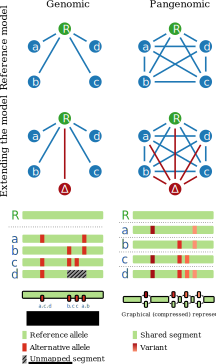
\includegraphics[width=0.8\textwidth]{figures/gen_vs_pang.pdf}
    \caption{\label{fig:genvpan} Genomic versus pangenomic sequence analysis patterns.
      Top left: In reference based genomic analyses, all genomes ($a \ldots f$) are compared to each other via their relationship to the reference genome $R$.
      Top right: In a pangenomic setting, we attempt to model direct relationships between all the genomes in our analysis, of which a particular reference $R$ is chosen arbitrarily.
      Bottom left: When extending our analysis with a new genome, $\Delta$, we add it to the genomic model by comparing it to reference $R$.
      Bottom right: In contrast, adding a new genome to a pangenomic analysis compares it directly with all other genomes in the model.
    }
\end{figure}

\begin{figure}[h!]
    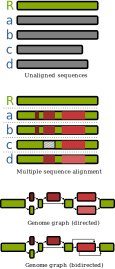
\includegraphics[width=0.5\textwidth]{figures/data_structures.pdf}
    \caption{\label{fig:models} Pangenomic models.
      A collection of sequences representing a pangenome, their alignment, a acyclic sequence graph representing the linear alignment, and a generic sequence grpah including an inversion.
    }
\end{figure}
